\documentclass[12pt]{article}

\usepackage{sbc-template}
\usepackage{graphicx,url}
\usepackage[utf8]{inputenc}
\usepackage[T1]{fontenc}
\usepackage[brazil]{babel}
\usepackage{amsmath,amssymb}
\usepackage{booktabs}
\usepackage{subcaption}

\graphicspath{{../results/figuras/}{../results/tinkercad/}{figuras/}}
% Gerado por experimentos/gera_macros.py -- não editar à mão
\newcommand{\CPU}{Intel64 Family 6 Model 183 Stepping 1, GenuineIntel}
\newcommand{\DcritHil}{55}
\newcommand{\DcritHilFino}{224}
\newcommand{\ErroAbAlUmZero}{9{,}3\times 10^{-12}}
\newcommand{\ErroAbAlDoisZero}{4{,}3\times 10^{-5}}
\newcommand{\ErroAbAlCinco}{1{,}4\times 10^{-13}}
\newcommand{\ErroAbWiUmZero}{3{,}6\times 10^{-10}}
\newcommand{\ErroAbWiDoisZero}{7{,}9\times 10^{-3}}
\newcommand{\ErroAbWiCinco}{1{,}2\times 10^{-14}}
\newcommand{\ErroCompAlUmZero}{1{,}5\times 10^{-11}}
\newcommand{\ErroCompAlDoisZero}{2{,}7\times 10^{-4}}
\newcommand{\ErroCompAlCinco}{5{,}1\times 10^{-13}}
\newcommand{\ErroCompWiUmZero}{6{,}0\times 10^{-10}}
\newcommand{\ErroCompWiDoisZero}{6{,}7\times 10^{-3}}
\newcommand{\ErroCompWiCinco}{5{,}6\times 10^{-14}}
\newcommand{\ErroPadeA}{2{,}7\times 10^{-1}}
\newcommand{\ErroPadeApct}{27{,}2}
\newcommand{\ErroPadeB}{7{,}4\times 10^{-3}}
\newcommand{\ErroPadeC}{1{,}3\times 10^{-4}}
\newcommand{\ErroPadeD}{1{,}3\times 10^{-6}}
\newcommand{\ErroPadeE}{8{,}2\times 10^{-9}}
\newcommand{\ErroTinkMax}{1{,}3\times 10^{-4}}
\newcommand{\FaixaDinMax}{2{,}0\times 10^{37}}
\newcommand{\KcritA}{60{,}00}
\newcommand{\KcritC}{8{,}571}
\newcommand{\KminB}{203{,}87}
\newcommand{\MAA}{0{,}422}
\newcommand{\MAB}{0{,}014}
\newcommand{\MAC}{0{,}874}
\newcommand{\MAD}{0{,}622}
\newcommand{\MFA}{44{,}5}
\newcommand{\MFB}{49{,}2}
\newcommand{\MFC}{48{,}4}
\newcommand{\MFD}{49{,}8}
\newcommand{\MFsemAtraso}{89{,}82}
\newcommand{\MGA}{9{,}54}
\newcommand{\MGB}{-5{,}85}
\newcommand{\MGC}{1{,}76}
\newcommand{\MGD}{5{,}75}
\newcommand{\MGlinA}{3{,}000}
\newcommand{\MGlinB}{0{,}510}
\newcommand{\MGlinC}{1{,}224}
\newcommand{\MGlinD}{1{,}939}
\newcommand{\NA}{0}
\newcommand{\NB}{-1}
\newcommand{\NC}{0}
\newcommand{\ND}{0}
\newcommand{\PA}{0}
\newcommand{\PB}{1}
\newcommand{\PC}{0}
\newcommand{\PD}{0}
\newcommand{\PtsA}{5998}
\newcommand{\PtsB}{5998}
\newcommand{\PtsC}{5998}
\newcommand{\PtsD}{6718}
\newcommand{\RobAbsErro}{37{,}3}
\newcommand{\RobAbsMin}{62{,}7}
\newcommand{\TAbAlUmZero}{939}
\newcommand{\TAbAlDoisZero}{3342}
\newcommand{\TAbAlCinco}{497}
\newcommand{\TAbWiUmZero}{1096}
\newcommand{\TAbWiDoisZero}{3380}
\newcommand{\TAbWiCinco}{421}
\newcommand{\TCompAlUmZero}{23}
\newcommand{\TCompAlDoisZero}{49}
\newcommand{\TCompAlCinco}{18}
\newcommand{\TCompWiUmZero}{25}
\newcommand{\TCompWiDoisZero}{51}
\newcommand{\TCompWiCinco}{19}
\newcommand{\TLugarAlUmZero}{139}
\newcommand{\TLugarAlDoisZero}{143}
\newcommand{\TLugarAlCinco}{144}
\newcommand{\TLugarWiUmZero}{119}
\newcommand{\TLugarWiDoisZero}{301}
\newcommand{\TLugarWiCinco}{86}
\newcommand{\TNyqAlUmZero}{0{,}74}
\newcommand{\TNyqAlDoisZero}{0{,}88}
\newcommand{\TNyqAlCinco}{0{,}52}
\newcommand{\TNyqWiUmZero}{0{,}67}
\newcommand{\TNyqWiDoisZero}{0{,}73}
\newcommand{\TNyqWiCinco}{0{,}54}
\newcommand{\TRouthAlUmZero}{83}
\newcommand{\TRouthAlDoisZero}{204}
\newcommand{\TRouthAlCinco}{43}
\newcommand{\TRouthWiUmZero}{89}
\newcommand{\TRouthWiDoisZero}{207}
\newcommand{\TRouthWiCinco}{48}
\newcommand{\TauCrit}{1{,}1220}
\newcommand{\TauCritBis}{1{,}1220}
\newcommand{\TauHil}{1{,}10}
\newcommand{\TauHilFino}{1{,}120}
\newcommand{\TauPadeA}{1{,}4269}
\newcommand{\TauPadeB}{1{,}1303}
\newcommand{\TauPadeC}{1{,}1221}
\newcommand{\TauPadeD}{1{,}1220}
\newcommand{\TauPadeE}{1{,}1220}
\newcommand{\TkUmD}{0}
\newcommand{\TkUmErro}{9{,}3\times 10^{-5}}
\newcommand{\TkUmPico}{1{,}000}
\newcommand{\TkDoisD}{25}
\newcommand{\TkDoisErro}{7{,}4\times 10^{-5}}
\newcommand{\TkDoisPico}{1{,}240}
\newcommand{\TkTresD}{50}
\newcommand{\TkTresErro}{7{,}8\times 10^{-5}}
\newcommand{\TkTresPico}{1{,}822}
\newcommand{\TkTresTaxa}{-0{,}047}
\newcommand{\TkQuatroaD}{54}
\newcommand{\TkQuatroaErro}{8{,}7\times 10^{-5}}
\newcommand{\TkQuatroaPico}{1{,}913}
\newcommand{\TkQuatroaTaxa}{-7{,}7\times 10^{-3}}
\newcommand{\TkQuatrobD}{55}
\newcommand{\TkQuatrobErro}{1{,}2\times 10^{-4}}
\newcommand{\TkQuatrobPico}{2{,}050}
\newcommand{\TkQuatrobTaxa}{9{,}0\times 10^{-4}}
\newcommand{\TkQuatrocD}{56}
\newcommand{\TkQuatrocErro}{8{,}7\times 10^{-5}}
\newcommand{\TkQuatrocPico}{2{,}687}
\newcommand{\TkQuatrocTaxa}{9{,}1\times 10^{-3}}
\newcommand{\TkCincoD}{60}
\newcommand{\TkCincoErro}{1{,}3\times 10^{-4}}
\newcommand{\TkCincoPico}{5{,}555}
\newcommand{\TkCincoTaxa}{0{,}038}
\newcommand{\TkSeisD}{44}
\newcommand{\TkSeisErro}{2{,}3\times 10^{-4}}
\newcommand{\TkSeisPico}{1{,}738}
\newcommand{\TkSeisTaxa}{-0{,}151}
\newcommand{\VerControl}{0.10.2}
\newcommand{\VerNumpy}{2.5.3}
\newcommand{\VerPython}{3.12.10}
\newcommand{\VerScipy}{1.18.1}
\newcommand{\WcfA}{3{,}317}
\newcommand{\WcfB}{0{,}000}
\newcommand{\WcfC}{1{,}558}
\newcommand{\WcfD}{2{,}708}
\newcommand{\WcgA}{1{,}838}
\newcommand{\WcgB}{61{,}274}
\newcommand{\WcgC}{0{,}966}
\newcommand{\WcgD}{1{,}397}


\sloppy

\title{Análise Computacional e Comparativa de Critérios de Estabilidade em Sistemas Dinâmicos: Nyquist, Routh-Hurwitz, Lugar das Raízes e Bode}

\author{Davi Valério de Oliveira\inst{1}, Luiz Iassuoo Yabagata Neto\inst{1},\\ Samuel André Lopes Furtado\inst{1}}

\address{Curso de Engenharia da Computação\\
  Pontifícia Universidade Católica de Goiás (PUC Goiás) -- Goiânia -- GO -- Brasil\\
  Disciplina de Controle de Processos -- Prof. Dr. Nilson Cardoso Amaral}

\begin{document}

\maketitle

\begin{abstract}
  This paper presents a tool, written from scratch in Python with NumPy, that assesses the stability of linear systems by the Nyquist criterion and compares it with Routh-Hurwitz, root locus and Bode analysis. On four benchmark systems (stable, open-loop unstable, non-minimum phase and a networked PID loop with delay) all methods agree on the gain boundary to nine digits and match python-control. The exact critical delay is \TauCrit~s, while a first-order Padé approximation errs by \ErroPadeApct\%. A two-Arduino hardware-in-the-loop setup simulated in Tinkercad confirms the prediction.
\end{abstract}

\begin{resumo}
  Este artigo apresenta uma ferramenta, implementada do zero em Python com NumPy, que avalia a estabilidade de sistemas lineares pelo critério de Nyquist e a compara com Routh-Hurwitz, Lugar das Raízes e Diagrama de Bode. Em quatro sistemas de teste (estável, instável em malha aberta, de fase não mínima e uma malha PID com atraso de rede), os métodos concordam na fronteira de ganho até a nona casa decimal e coincidem com a biblioteca python-control. O atraso crítico exato é de \TauCrit~s, enquanto a aproximação de Padé de primeira ordem erra em \ErroPadeApct\%. Uma montagem \textit{hardware-in-the-loop} com dois Arduinos, simulada no Tinkercad, confirma a previsão.
\end{resumo}

% ======================================================================
\section{Introdução}

A análise de estabilidade é etapa obrigatória no projeto de sistemas de controle, de sistemas embarcados e de laços fechados por redes de comunicação. Os critérios clássicos respondem a perguntas diferentes. O critério de Routh-Hurwitz decide, por álgebra sobre os coeficientes, se todas as raízes da equação característica estão no semiplano esquerdo, mas não informa o quanto o sistema está próximo da instabilidade. O Lugar das Raízes mostra como os polos de malha fechada se movem com o ganho, e o Diagrama de Bode e o critério de Nyquist trabalham no domínio da frequência e fornecem margens de estabilidade relativa \cite{ogata2010,nise2017}.

O critério de Nyquist \cite{nyquist1932} tem duas propriedades de interesse computacional: aplica-se diretamente a plantas instáveis em malha aberta e trata o atraso de transporte $e^{-\tau s}$ sem aproximação, pois só exige avaliar a função de malha aberta sobre um contorno. Em sistemas controlados via rede, nos quais o atraso de comunicação é intrínseco \cite{zhang2001}, essa propriedade é decisiva. Os métodos que operam sobre polinômios em $s$ exigem substituir o atraso por uma função racional, tipicamente a aproximação de Padé \cite{pade1892}.

Para estudantes de Engenharia da Computação, o desafio inclui a implementação: amostrar adequadamente o contorno, contar envoltórios de forma robusta, lidar com polos sobre o eixo imaginário e controlar erros de arredondamento quando a ordem cresce. Este trabalho desenvolve e avalia empiricamente essa implementação.

\subsection{Objetivos}

O objetivo geral é desenvolver uma ferramenta computacional para analisar a estabilidade de sistemas lineares invariantes no tempo pelo critério de Nyquist e comparar seus resultados, limitações e desempenho com Routh-Hurwitz, Lugar das Raízes e Bode. Os objetivos específicos são:
(i) implementar o critério de Nyquist a partir do Princípio do Argumento;
(ii) extrair automaticamente as margens de ganho e de fase;
(iii) implementar Routh-Hurwitz, com seus casos especiais, e o Lugar das Raízes sem bibliotecas de controle;
(iv) quantificar a vantagem do tratamento exato do atraso frente às aproximações de Padé;
(v) medir tempo de execução e erro numérico em função da ordem do sistema; e
(vi) aplicar o critério para prever o atraso crítico de um laço PID em uma montagem \textit{hardware-in-the-loop} (HIL) com microcontroladores.

As contribuições são: o código aberto e testado; a validação empírica, sistema a sistema, da tabela comparativa proposta no enunciado do projeto; e um estudo de estabilidade numérica que documenta uma falha real de implementação do critério de Routh e sua correção.

% ======================================================================
\section{Fundamentação teórica}

\subsection{Princípio do Argumento e mapeamento conforme}

Seja $F(s)$ uma função racional e $\Gamma$ um contorno fechado simples no plano $s$, percorrido no sentido horário, que não passa por zeros nem polos de $F$. O Princípio do Argumento de Cauchy estabelece que a imagem $F(\Gamma)$ envolve a origem, no sentido horário,
\begin{equation}
  N = Z - P
  \label{eq:argumento}
\end{equation}
vezes, em que $Z$ e $P$ são, respectivamente, o número de zeros e de polos de $F$ no interior de $\Gamma$. O resultado decorre da variação do argumento de $F(s)=K\prod(s-z_i)/\prod(s-p_j)$: cada fator $(s-z_i)$ com $z_i$ interno a $\Gamma$ contribui com uma volta completa de $-2\pi$, enquanto fatores com raízes externas têm variação líquida nula. Como $F$ é analítica fora de seus polos, o mapeamento é conforme (preserva ângulos) em todo ponto regular, o que garante que a curva imagem é contínua e que a contagem de voltas é bem definida \cite{astrom2008}.

\subsection{Critério de estabilidade de Nyquist}

Para um laço com realimentação negativa e função de malha aberta $L(s)=G(s)H(s)$, os polos de malha fechada são os zeros de $F(s)=1+L(s)$, e os polos de $F$ coincidem com os de $L$. Escolhendo $\Gamma$ como o contorno de Nyquist, que sobe pelo eixo imaginário de $-jR$ a $+jR$ e se fecha por um semicírculo de raio $R\to\infty$ no semiplano direito (SPD), a Eq.~\eqref{eq:argumento} aplicada a $F$ dá
\begin{equation}
  Z = N + P,
  \label{eq:nyquist}
\end{equation}
em que $Z$ é o número de polos de malha fechada no SPD, $P$ o número de polos de $L$ no SPD e $N$ o número de envoltórios horários de $L(\Gamma)$ em torno do ponto crítico $-1+j0$ (pois envolver a origem com $1+L$ equivale a envolver $-1$ com $L$). A malha fechada é estável se, e somente se, $Z=0$, isto é, $N=-P$: o diagrama deve envolver $-1$ no sentido anti-horário tantas vezes quantos forem os polos instáveis de malha aberta \cite{nyquist1932,ogata2010}.

Polos de $L$ sobre o eixo $j\omega$ (integradores ou pares $\pm j\omega_0$) violam a hipótese do Princípio do Argumento. O tratamento usual é desviar o contorno por semicírculos de raio $r\to 0$ pela direita, o que exclui esses polos do interior de $\Gamma$ e, portanto, da contagem de $P$. Cada desvio é mapeado em um arco de raio $\to\infty$ no plano $L$ \cite{astrom2008}.

\subsection{Margens de estabilidade}

A estabilidade relativa é medida pela distância de $L(j\omega)$ ao ponto crítico. Sendo $\omega_{cf}$ a frequência em que $\angle L(j\omega_{cf})=-180^\circ$ e $\omega_{cg}$ aquela em que $|L(j\omega_{cg})|=1$, definem-se a margem de ganho e a margem de fase
\begin{equation}
  \mathrm{MG} = \frac{1}{|L(j\omega_{cf})|}, \qquad
  \mathrm{MF} = 180^\circ + \angle L(j\omega_{cg}).
\end{equation}
Um atraso adicional $\Delta\tau$ multiplica $L$ por $e^{-j\omega\Delta\tau}$, que não altera o módulo e reduz a fase em $\omega\Delta\tau$. O maior atraso tolerado, a margem de atraso, é então $\mathrm{MA}=\mathrm{MF}/\omega_{cg}$ (com MF em radianos). Para $P>0$, as margens devem ser interpretadas à luz do critério completo, pois a perda de estabilidade pode ocorrer tanto pelo aumento quanto pela redução do ganho \cite{skogestad2005}.

\subsection{Sistemas com atraso de transporte}

O atraso puro $e^{-\tau s}$ é transcendente, de modo que $1+L(s)=0$ passa a ter infinitas raízes. No critério de Nyquist isso não traz dificuldade: basta avaliar $e^{-j\omega\tau}$ sobre o contorno, cujo módulo é unitário no eixo e limitado por $1$ no SPD. Já os métodos baseados em polinômios exigem uma aproximação racional. A aproximação de Padé de ordem $[N/N]$ \cite{pade1892} é
\begin{equation}
  e^{-\tau s} \approx \frac{\sum_{k=0}^{N} c_k(-\tau s)^k}{\sum_{k=0}^{N} c_k(\tau s)^k},
  \qquad c_k=\frac{(2N-k)!\,N!}{(2N)!\,k!\,(N-k)!}.
  \label{eq:pade}
\end{equation}
Ela é um passa-tudo exato em módulo, mas seu erro de fase cresce com $\omega\tau$; além disso, introduz $N$ zeros no SPD e eleva o grau da equação característica em $N$.

\subsection{Métodos alternativos}

\textbf{Routh-Hurwitz.} Para $a_n s^n+\cdots+a_0$, a tabela de Routh é construída a partir das duas primeiras linhas (coeficientes alternados) pela recorrência $b_j=(b_0a_{j+1}-a_0b_{j+1})/b_0$, e o número de raízes no SPD é igual ao número de trocas de sinal da primeira coluna \cite{routh1877,hurwitz1895}. Há dois casos especiais: um zero na primeira coluna de uma linha não nula, tratado substituindo-o por $\varepsilon\to 0^+$; e uma linha inteiramente nula, que indica raízes simétricas em relação à origem e é tratada substituindo-a pelos coeficientes da derivada do polinômio auxiliar formado pela linha anterior \cite{nise2017}.

\textbf{Lugar das Raízes.} Para $L(s)=KN(s)/D(s)$, o lugar é o conjunto das raízes de $D(s)+KN(s)=0$ com $K\in[0,\infty)$ \cite{evans1948}. As regras de construção fornecem o centroide das assíntotas, $\sigma_a=(\sum p_i-\sum z_i)/(n-m)$, seus ângulos, $(2k+1)180^\circ/(n-m)$, e os pontos de separação, que são raízes reais de $N D' - N' D = 0$ com $K>0$.

\textbf{Diagrama de Bode.} Representa $20\log_{10}|L(j\omega)|$ e $\angle L(j\omega)$ em escala logarítmica de frequência \cite{bode1945}. A aproximação assintótica usa retas de $\pm 20$~dB/década por raiz real e $\pm 40$~dB/década por par complexo a partir das frequências de quebra; o atraso contribui apenas com $-\omega\tau$ na fase.

% ======================================================================
\section{Metodologia e arquitetura computacional}

\subsection{Arquitetura}

A ferramenta é um pacote Python (\texttt{src/estabilidade}) organizado em módulos independentes: polinômios (Horner, derivada e produto), raízes, função de transferência, Nyquist, margens, Bode, Padé, Routh-Hurwitz, Lugar das Raízes, simulação no tempo e gêmeo digital do HIL. Conforme exigido, nenhum algoritmo de controle é delegado a bibliotecas prontas: o NumPy \cite{harris2020} é usado para vetores, aritmética complexa e autovalores. As bibliotecas python-control \cite{fuller2021} e SciPy \cite{virtanen2020} aparecem apenas na suíte de testes e nos scripts de validação cruzada. Todos os números, tabelas e figuras deste artigo são gerados por scripts em \texttt{experimentos/} e incluídos no texto sem transcrição manual. O código-fonte, a suíte de testes e as instruções de reprodução estão no repositório do projeto\footnote{\url{https://github.com/liassuo/controle-processos}}.

O tipo central é \texttt{FT(num, den, atraso)}, que representa $L(s)=N(s)/D(s)\cdot e^{-\tau s}$ e é avaliado pelo método de Horner, com o termo exponencial calculado diretamente. Os métodos no plano $s$ recusam explicitamente funções com atraso e exigem a conversão prévia por Padé, o que torna a assimetria entre os métodos visível no próprio código.

\subsection{Algoritmos}

\textbf{Contorno e envoltórios.} Os polos de $L$ são classificados em SPD, SPE e eixo imaginário. O raio $R$ do semicírculo externo é escolhido por uma cota sobre o módulo das raízes, $|L(s)|\le |b_m/a_n|\prod(R+|z_i|)/\prod(R-|p_j|) < 1/2$, que também vale com atraso porque $|e^{-\tau s}|\le 1$ no SPD. Onde $|L|<1/2$, o ponto $L+1$ permanece no semiplano $\mathrm{Re}>0$ e não contribui com voltas, o que justifica truncar o refinamento em altas frequências. O ramo $\omega>0$ é amostrado em escala logarítmica e refinado por bissecção sempre que a variação do ângulo de $L+1$ entre amostras vizinhas excede $15^\circ$; com atraso, impõe-se ainda $\Delta\omega\,\tau\le 0{,}2$ rad, pois o diagrama espirala. O ramo $\omega<0$ é obtido por simetria conjugada, e os polos no eixo recebem semicírculos de raio $10^{-4}$. O número de voltas é calculado de duas formas independentes: pela soma dos ângulos $\sum \arg[(L_{k+1}+1)/(L_k+1)]/2\pi$ e pela contagem de cruzamentos com sinal de uma semirreta horizontal a partir de $-1$, que tem custo $O(n)$ e não depende de funções trigonométricas \cite{hormann2001}. A implementação exige que as duas contagens coincidam.

\textbf{Margens.} Os cruzamentos de ganho e de fase são isolados em uma grade logarítmica de $2\times 10^5$ pontos entre $10^{-4}$ e $10^4$~rad/s e refinados por bissecção. A fase é desdobrada continuamente na parte racional e acrescida exatamente de $-\omega\tau$. O caso $\omega_{cf}=0$, típico de $P>0$, é tratado à parte.

\textbf{Routh-Hurwitz.} Antes da tabela, o polinômio é escalonado em frequência ($s\to\alpha s$, com $\alpha=|a_0/a_n|^{1/n}$), o que preserva o sinal da parte real das raízes. Um elemento é considerado nulo quando é desprezível diante dos termos que o geraram, $|b_j|\le 64\,n\,u\,(|b_0a_{j+1}|+|a_0b_{j+1}|)/|b_0|$, em que $u$ é o épsilon de máquina. A Seção~\ref{sec:robustez} mostra por que esse critério relativo ao cancelamento é necessário.

\textbf{Raízes.} São implementados dois métodos: os autovalores da matriz companheira, $O(n^3)$, princípio também usado por \texttt{numpy.roots} \cite{edelman1995}; e a iteração simultânea de Aberth-Ehrlich, $O(n^2)$ por iteração, programada do zero com estimativas iniciais pela cota de Fujiwara e parada por erro regressivo, isto é, quando $|p(z)|\le u\sum|a_k||z|^k$.

\textbf{Lugar das Raízes.} O ganho $K$ é varrido com passo adaptativo, que é reduzido quando alguma raiz se desloca mais que 2\% da escala do problema; os ramos são mantidos contínuos por emparelhamento com o vizinho mais próximo. Os cruzamentos do eixo $j\omega$ são refinados por bissecção sobre a maior parte real.

\subsection{Sistemas de teste}

A Tabela~\ref{tab:sistemas} resume os quatro sistemas, definidos em \texttt{sistemas.py}. O Sistema B usa o modelo linearizado do levitador magnético, $m\ddot{x}=mg-c\,i^2/x^2$, que em torno de $(x_0,i_0)$ resulta em $G(s)=(2g/i_0)/(s^2-2g/x_0)$, com polos em $\pm\sqrt{2g/x_0}$. Os parâmetros foram escolhidos de modo que o polo instável fique em $20$~rad/s ($x_0=2g/400\approx 4{,}9$~cm, $i_0=1$~A). O Sistema D é o mesmo laço usado na montagem HIL: um PID com derivada filtrada, $C(s)=K_p+K_i/s+K_ds/(T_fs+1)$, com $K_p=2$, $K_i=1$, $K_d=0{,}5$ e $T_f=0{,}1$~s, sobre um processo de segunda ordem, com atraso nominal de rede $\tau=0{,}5$~s.

\begin{table}[ht]
\centering
\caption{Sistemas de teste (realimentação negativa unitária).}
\label{tab:sistemas}
\small
\begin{tabular}{lll}
\toprule
Sistema & $L(s)$ & Característica \\
\midrule
A & $\dfrac{20}{(s+1)(s+2)(s+3)}$ & estável em malha aberta, 3ª ordem \\[2mm]
B & $\dfrac{400(s+10)}{s+100}\cdot\dfrac{19{,}62}{s^2-400}$ & levitador instável ($P=1$) com avanço de fase \\[2mm]
C & $\dfrac{7(1-s)}{(s+1)(s+2)(s+3)}$ & fase não mínima (zero em $s=+1$) \\[2mm]
D & $C_{PID}(s)\,\dfrac{1}{(s+1)(0{,}5s+1)}\,e^{-0{,}5s}$ & atraso de transporte (rede) \\
\bottomrule
\end{tabular}
\end{table}

\subsection{Protocolo de validação e de desempenho}

A correção é verificada em três níveis. O primeiro são 74 testes unitários com resultados analíticos conhecidos, como o ganho crítico de $60$ do Sistema A, o limite $\tau_{crit}=2\pi/(3\sqrt{3})$ para $2e^{-\tau s}/(s+1)$, os casos especiais clássicos de Routh e os polinômios de Padé de alta ordem. O segundo é a validação cruzada das margens, dos envoltórios, dos polos de malha fechada e dos polinômios de Padé com o python-control (versão \VerControl) e da resposta em frequência com o SciPy (versão \VerScipy). O terceiro é a simulação temporal independente, por Runge-Kutta de quarta ordem com atraso, que confirma cada veredito de estabilidade.

Para a escalabilidade, foram usadas duas famílias de polinômios com raízes conhecidas e semente fixa: raízes estáveis aleatórias com $\mathrm{Re}\in[-10;-0{,}1]$ e a família de Wilkinson, com raízes $-1,-2,\dots,-n$, conhecida por seu mau condicionamento \cite{wilkinson1984}. Mediu-se o tempo mediano de 7 repetições para $n$ de 2 a 30, com destaque para $n=5$, $10$ e $20$, conforme o enunciado, em Python \VerPython\ e NumPy \VerNumpy\ (processador \CPU).

\subsection{Montagem \textit{hardware-in-the-loop} no Tinkercad}
\label{sec:met-hil}

Na trilha de Engenharia da Computação, o laço do Sistema D foi implementado em dois Arduinos Uno simulados no Tinkercad Circuits. O Arduino ``Planta'' atua como relógio mestre ($T_s=20$~ms): integra a planta discretizada por segurador de ordem zero (ZOH) e emula a rede com um \textit{buffer} circular. O atraso é ajustado por um potenciômetro, que define $d$ amostras e, portanto, $\tau=d\,T_s$, e uma chave deslizante ativa um atraso variável sorteado em $[d,d+20]$. Os comandos são entregues em ordem, sem reordenação de pacotes. O Arduino ``Controlador'' executa o PID discretizado por Euler para trás, com saturação em $\pm 10$ e \textit{antiwindup} condicional. As placas trocam mensagens de texto pela serial de hardware a 115\,200~bit/s. Um gêmeo digital em Python reproduz o mesmo algoritmo, em ponto flutuante de 32 bits, e um teste automatizado garante que as constantes dos \textit{sketches} coincidem com as do gêmeo.

% ======================================================================
\section{Resultados}

\subsection{Análise dos quatro sistemas}
\label{sec:res-sistemas}

A Tabela~\ref{tab:resultados} e a Figura~\ref{fig:nyquist} resumem a análise. Em todos os casos, as duas contagens de envoltórios coincidiram e o veredito de Nyquist ($Z=0$) concordou com o número de raízes no SPD dado pelo Routh, que no Sistema D foi aplicado sobre a aproximação de Padé de ordem 3, e com a simulação temporal.

\begin{table}[ht]
\centering
\caption{Resultados por sistema: Nyquist ($P$, $N$, $Z$), margens (frequências em rad/s), número de raízes no SPD pelo Routh e veredito da simulação temporal.}
\label{tab:resultados}
\small
\resizebox{\textwidth}{!}{\begin{tabular}{lcccccccccc}
\hline
Sist. & $P$ & $N$ & $Z$ & MG (dB) & $\omega_{cf}$ & MF (°) & $\omega_{cg}$ & MA (s) & Routh SPD & Simulação \\
\hline
A & 0 & 0 & 0 & 9{,}54 & 3{,}317 & 44{,}46 & 1{,}838 & 0{,}422 & 0 & estável \\
B & 1 & -1 & 0 & -5{,}85 & 0{,}000 & 49{,}23 & 61{,}274 & 0{,}014 & 0 & estável \\
C & 0 & 0 & 0 & 1{,}76 & 1{,}558 & 48{,}36 & 0{,}966 & 0{,}874 & 0 & estável \\
D & 0 & 0 & 0 & 5{,}75 & 2{,}708 & 49{,}79 & 1{,}397 & 0{,}622 & 0 & estável \\
\hline
\end{tabular}
}
\end{table}

\begin{figure}[ht]
\centering
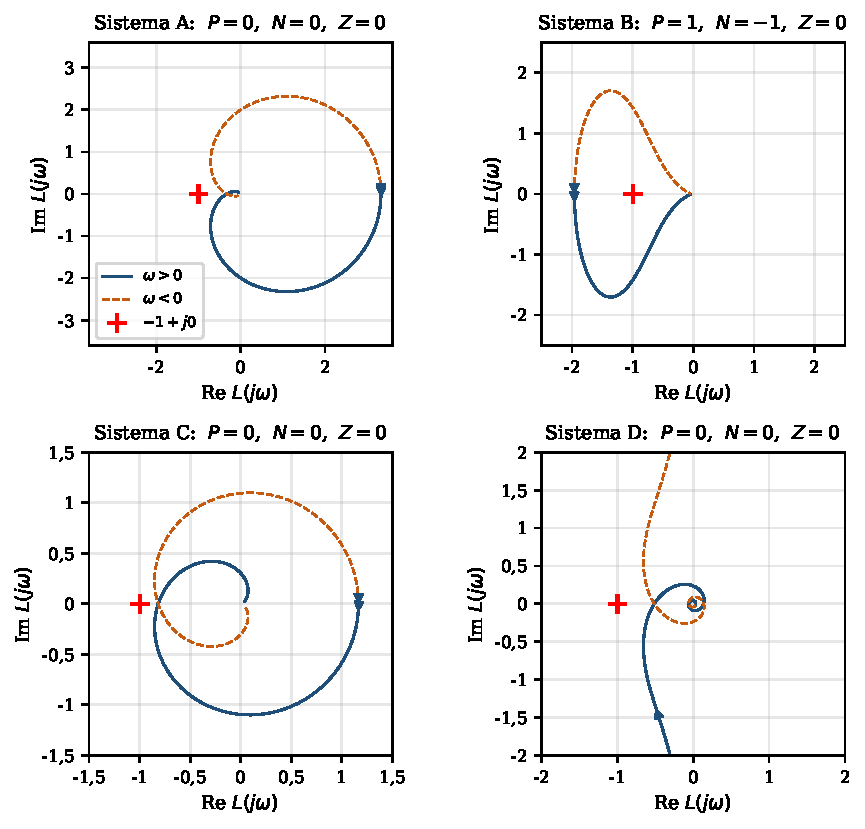
\includegraphics[width=0.92\textwidth]{nyquist_sistemas.pdf}
\caption{Diagramas de Nyquist calculados pela ferramenta. As setas indicam $\omega$ crescente e a cruz marca $-1+j0$. No Sistema B ($P=1$), o diagrama envolve $-1$ uma vez no sentido anti-horário ($N=-1$), logo $Z=0$.}
\label{fig:nyquist}
\end{figure}

O \textbf{Sistema A} é o caso de referência: com MG de \MGA~dB, o ganho pode ser multiplicado por \MGlinA\ antes da instabilidade, o que corresponde a $K_{crit}=\KcritA$, exatamente o valor analítico. O \textbf{Sistema B} ilustra o caso $P>0$: a estabilidade exige que o diagrama envolva $-1$ no sentido anti-horário, e a margem de ganho é \emph{negativa} em dB (\MGB~dB). Isso significa que a malha se torna instável se o ganho for \emph{reduzido} abaixo de $K_{min}=\KminB$, interpretação que o Diagrama de Bode isolado não fornece. O \textbf{Sistema C} tem o mesmo módulo $|L(j\omega)|$ que o seu gêmeo de fase mínima $7(1+s)/[(s+1)(s+2)(s+3)]$, mas o zero no SPD acrescenta atraso de fase e limita o ganho a $\KcritC$, enquanto o gêmeo de fase mínima é estável para qualquer $K>0$. O \textbf{Sistema D} tem MF de \MFD$^\circ$ e margem de atraso de \MAD~s, isto é, tolera um atraso total de $0{,}5+\MAD=\TauCrit$~s.

As Figuras~\ref{fig:bode} e~\ref{fig:lugar} mostram os diagramas de Bode (exato e assintótico) e o Lugar das Raízes. A Tabela~\ref{tab:ganho} compara a fronteira de estabilidade em $K$, normalizada pelo ganho nominal, obtida independentemente por Routh (bissecção sobre o veredito da tabela), pelo Lugar das Raízes (cruzamento do eixo $j\omega$) e pela margem de ganho de Nyquist/Bode. Nos sistemas racionais, os três métodos concordam até a nona casa decimal. No Sistema D, a pequena diferença entre Routh/Lugar e Nyquist é o erro da aproximação de Padé de ordem~3, e não do método.

\begin{figure}[ht]
\centering
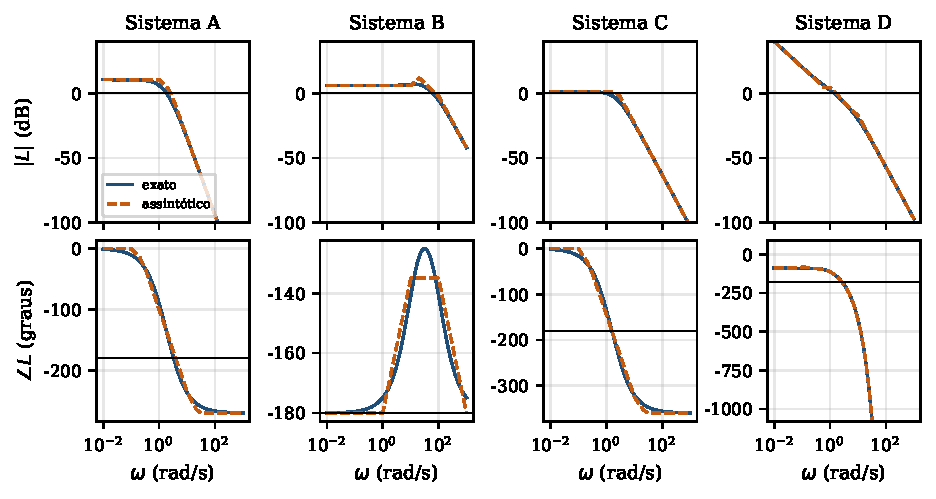
\includegraphics[width=\textwidth]{bode_sistemas.pdf}
\caption{Diagramas de Bode exatos (linha contínua) e aproximações assintóticas (tracejado). No Sistema D, a fase decresce sem limite por causa de $-\omega\tau$.}
\label{fig:bode}
\end{figure}

\begin{figure}[ht]
\centering
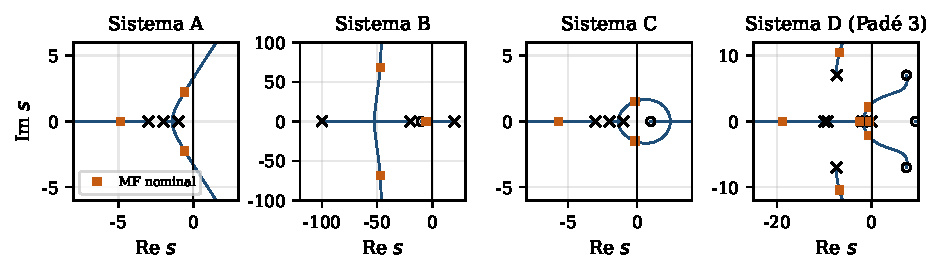
\includegraphics[width=\textwidth]{lugar_raizes_sistemas.pdf}
\caption{Lugar das Raízes ($\times$: polos; $\circ$: zeros; quadrados: polos de malha fechada no ganho nominal). Para o Sistema D, o lugar foi traçado sobre a aproximação de Padé de ordem 3, cujos zeros no SPD são visíveis.}
\label{fig:lugar}
\end{figure}

\begin{table}[ht]
\centering
\caption{Fronteira de estabilidade em $K$ (múltiplo do ganho nominal) por método.}
\label{tab:ganho}
\small
\begin{tabular}{lcccc}
\hline
Sist. & Routh & Lugar das Raízes & Nyquist/Bode (MG) & Tipo de limite \\
\hline
A & 3{,}00000 & 3{,}00000 & 3{,}00000 & máximo \\
B & 0{,}50968 & 0{,}50968 & 0{,}50968 & mínimo \\
C & 1{,}22449 & 1{,}22449 & 1{,}22449 & máximo \\
D & 1{,}93911 & 1{,}93911 & 1{,}93902 & máximo \\
\hline
\end{tabular}

\end{table}

\subsection{Validação cruzada}

A Tabela~\ref{tab:validacao} confronta os resultados próprios com o python-control. As margens coincidem até a quarta casa decimal mostrada, o número de envoltórios é idêntico e os polos de malha fechada diferem em no máximo $10^{-13}$. Para o Sistema D, a biblioteca não aceita atraso exato na função \texttt{margin}, de modo que a margem de fase de referência foi obtida descontando $\omega_{cg}\tau$ da margem do sistema sem atraso, o que é exato porque o atraso não altera o módulo.

\begin{table}[ht]
\centering
\caption{Validação cruzada com python-control.}
\label{tab:validacao}
\scriptsize
\resizebox{\textwidth}{!}{\begin{tabular}{lccccccc}
\hline
Sist. & MF própria (°) & MF python-control (°) & MG própria & MG python-control & $N$ própria & $N$ python-control & erro polos MF \\
\hline
A & 44{,}4630 & 44{,}4630 & 3{,}0000 & 3{,}0000 & 0 & 0 & 2{,}5e-15 \\
B & 49{,}2334 & 49{,}2334 & 0{,}5097 & 0{,}5097 & -1 & -1 & 4{,}3e-14 \\
C & 48{,}3587 & 48{,}3587 & 1{,}2245 & 1{,}2245 & 0 & 0 & 1{,}8e-15 \\
D & 49{,}7926 & 49{,}7926 & 1{,}9390 & -- & 0 & -- & 2{,}8e-14 \\
\hline
\end{tabular}
}
\end{table}

\subsection{Atraso exato versus aproximação de Padé}

O atraso crítico do Sistema D foi obtido de duas formas pelo tratamento exato: pela margem de atraso (\TauCrit~s) e por bissecção sobre o veredito $Z$ do Nyquist (\TauCritBis~s). Em seguida, substituiu-se $e^{-\tau s}$ por Padé de ordem $N$ e buscou-se o $\tau$ crítico por bissecção sobre o veredito de Routh e, independentemente, sobre as raízes da equação característica (Tabela~\ref{tab:pade}). A aproximação de primeira ordem superestima o atraso tolerável em \ErroPadeApct\%, um erro perigoso porque está do lado não conservador. O erro cai para $\ErroPadeB$ com $N=2$ e para $\ErroPadeC$ com $N=3$; a partir de $N=6$, a diferença fica abaixo da tolerância da bissecção (Figura~\ref{fig:pade}).

\begin{table}[ht]
\centering
\caption{Atraso crítico do Sistema D com aproximações de Padé (valor exato: \TauCrit~s).}
\label{tab:pade}
\small
\begin{tabular}{lccccc}
\hline
Ordem $N$ & Grau eq. caract. & $\tau_{crit}$ Routh (s) & $\tau_{crit}$ raízes (s) & Erro relativo & Tempo (ms) \\
\hline
1 & 5 & 1{,}426925 & 1{,}426925 & $2{,}72 \times 10^{-1}$ & 3{,}7 \\
2 & 6 & 1{,}130332 & 1{,}130332 & $7{,}44 \times 10^{-3}$ & 4{,}0 \\
3 & 7 & 1{,}122132 & 1{,}122132 & $1{,}34 \times 10^{-4}$ & 4{,}2 \\
4 & 8 & 1{,}121984 & 1{,}121984 & $1{,}34 \times 10^{-6}$ & 4{,}5 \\
5 & 9 & 1{,}121982 & 1{,}121982 & $8{,}23 \times 10^{-9}$ & 5{,}8 \\
6 & 10 & 1{,}121982 & 1{,}121982 & $1{,}39 \times 10^{-10}$ & 5{,}1 \\
7 & 11 & 1{,}121982 & 1{,}121982 & $1{,}39 \times 10^{-10}$ & 6{,}3 \\
8 & 12 & 1{,}121982 & 1{,}121982 & $1{,}39 \times 10^{-10}$ & 5{,}9 \\
9 & 13 & 1{,}121982 & 1{,}121982 & $1{,}39 \times 10^{-10}$ & 6{,}1 \\
10 & 14 & 1{,}121982 & 1{,}121982 & $1{,}39 \times 10^{-10}$ & 6{,}7 \\
11 & 15 & 1{,}121982 & 1{,}121982 & $1{,}39 \times 10^{-10}$ & 7{,}1 \\
12 & 16 & 1{,}121982 & 1{,}121982 & $1{,}39 \times 10^{-10}$ & 7{,}3 \\
\hline
\end{tabular}

\end{table}

\begin{figure}[ht]
\centering
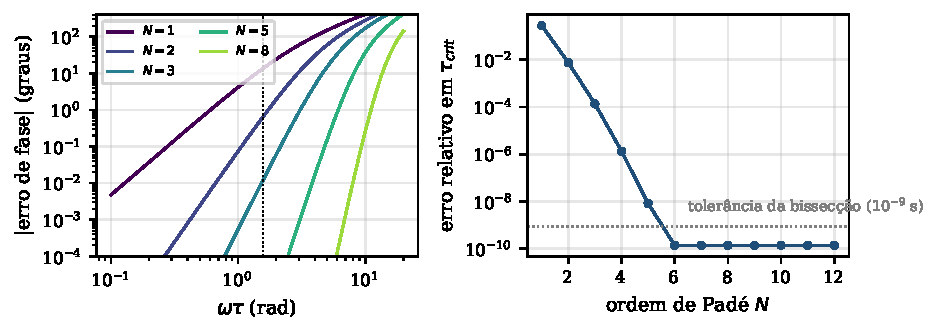
\includegraphics[width=\textwidth]{pade_erro.pdf}
\caption{Esquerda: erro de fase de Padé em função de $\omega\tau$ (a linha pontilhada marca $\omega_{cg}\tau_{crit}$). Direita: erro relativo no atraso crítico em função da ordem.}
\label{fig:pade}
\end{figure}

O custo dessa precisão é estrutural: cada ordem de Padé acrescenta um grau à equação característica e $N$ zeros ao SPD, e a faixa dinâmica dos coeficientes cresce rapidamente, chegando a $\FaixaDinMax$ para $N=20$, o que afeta diretamente a estabilidade numérica dos métodos algébricos.

\subsection{Estabilidade numérica do critério de Routh}
\label{sec:robustez}

A primeira versão da tabela de Routh considerava nulo qualquer elemento com $|b_j|\le 10^{-12}\max|a_k|$. Ao repetir o estudo de Padé para ordens altas, o Routh passou a acusar instabilidade em casos estáveis, em desacordo com as raízes. A causa é que, com coeficientes espalhados por dezenas de ordens de grandeza, elementos legítimos, mas pequenos, eram confundidos com zeros e substituídos por $\varepsilon$, o que alterava o sinal da primeira coluna. A Tabela~\ref{tab:robustez} quantifica o efeito sobre 300 valores de $\tau$ por ordem: com a tolerância absoluta e sem escalonamento, a concordância com as raízes cai para \RobAbsMin\%. Tanto o escalonamento de frequência quanto o critério relativo ao cancelamento, isoladamente, restauram 100\% de concordância até $N=20$ (grau 44); a versão final usa os dois.

\begin{table}[ht]
\centering
\caption{Concordância (\%) entre o veredito de Routh e o das raízes, por critério de zero numérico e uso de escalonamento (300 valores de $\tau$ por ordem $N$).}
\label{tab:robustez}
\small
\begin{tabular}{lccccc}
\hline
$N$ & Faixa dinâmica & Absoluta & Absoluta + esc. & Cancelamento & Cancel. + esc. \\
\hline
1 & $2{,}3 \times 10^{2}$ & 100{,}0 & 100{,}0 & 100{,}0 & 100{,}0 \\
3 & $5{,}5 \times 10^{4}$ & 100{,}0 & 100{,}0 & 100{,}0 & 100{,}0 \\
5 & $5{,}5 \times 10^{7}$ & 100{,}0 & 100{,}0 & 100{,}0 & 100{,}0 \\
6 & $2{,}4 \times 10^{9}$ & 99{,}7 & 100{,}0 & 100{,}0 & 100{,}0 \\
7 & $1{,}3 \times 10^{11}$ & 98{,}0 & 100{,}0 & 100{,}0 & 100{,}0 \\
8 & $7{,}6 \times 10^{12}$ & 94{,}7 & 100{,}0 & 100{,}0 & 100{,}0 \\
10 & $3{,}9 \times 10^{16}$ & 82{,}0 & 100{,}0 & 100{,}0 & 100{,}0 \\
12 & $3{,}0 \times 10^{20}$ & 62{,}7 & 100{,}0 & 100{,}0 & 100{,}0 \\
15 & $3{,}8 \times 10^{26}$ & 62{,}7 & 100{,}0 & 100{,}0 & 100{,}0 \\
20 & $2{,}0 \times 10^{37}$ & 62{,}7 & 100{,}0 & 100{,}0 & 100{,}0 \\
\hline
\end{tabular}

\end{table}

\subsection{Escalabilidade e custo computacional}

A Tabela~\ref{tab:escala} e a Figura~\ref{fig:escala} resumem o desempenho. O Routh, com custo $O(n^2)$ em Python puro, leva de \TRouthAlCinco~$\mu$s ($n=5$) a \TRouthAlDoisZero~$\mu$s ($n=20$). As raízes pela matriz companheira são mais rápidas em tempo absoluto, apesar do custo $O(n^3)$, porque o cálculo é delegado ao LAPACK compilado, enquanto o Aberth, $O(n^2)$ por iteração em Python vetorizado, fica entre \TAbAlCinco\ e \TAbAlDoisZero~$\mu$s. O Nyquist completo custa menos de 1~ms e é quase independente de $n$, porque o custo é dominado pelo número de pontos do contorno, e não pela ordem. O cálculo de margens é o mais caro dentre os métodos de frequência (dezenas de milissegundos) apenas pela grade densa adotada, e o Lugar das Raízes é o mais caro de todos (centenas de milissegundos), por resolver um problema de raízes a cada passo de $K$.

\begin{table}[ht]
\centering
\caption{Tempo mediano e erro relativo máximo das raízes para $n=5$, $10$ e $20$.}
\label{tab:escala}
\scriptsize
\resizebox{\textwidth}{!}{\begin{tabular}{llccccccccc}
\hline
Família & $n$ & Routh ($\mu$s) & Compan. ($\mu$s) & Aberth ($\mu$s) & Nyquist (ms) & Margens (ms) & Lugar (ms) & Erro compan. & Erro Aberth & Routh ok \\
\hline
aleatória & 5 & 42{,}7 & 18{,}2 & 497{,}0 & 0{,}52 & 42{,}3 & 144 & $5{,}1 \times 10^{-13}$ & $1{,}4 \times 10^{-13}$ & sim \\
aleatória & 10 & 82{,}7 & 23{,}1 & 938{,}6 & 0{,}74 & 54{,}0 & 139 & $1{,}5 \times 10^{-11}$ & $9{,}3 \times 10^{-12}$ & sim \\
aleatória & 20 & 204{,}3 & 49{,}5 & 3342{,}5 & 0{,}88 & 87{,}6 & 143 & $2{,}7 \times 10^{-4}$ & $4{,}3 \times 10^{-5}$ & sim \\
Wilkinson & 5 & 48{,}2 & 18{,}6 & 421{,}0 & 0{,}54 & 38{,}2 & 86 & $5{,}6 \times 10^{-14}$ & $1{,}2 \times 10^{-14}$ & sim \\
Wilkinson & 10 & 88{,}8 & 24{,}7 & 1095{,}6 & 0{,}67 & 53{,}4 & 119 & $6{,}0 \times 10^{-10}$ & $3{,}6 \times 10^{-10}$ & sim \\
Wilkinson & 20 & 207{,}1 & 50{,}9 & 3379{,}9 & 0{,}73 & 84{,}6 & 301 & $6{,}7 \times 10^{-3}$ & $7{,}9 \times 10^{-3}$ & sim \\
\hline
\end{tabular}
}
\end{table}

\begin{figure}[ht]
\centering
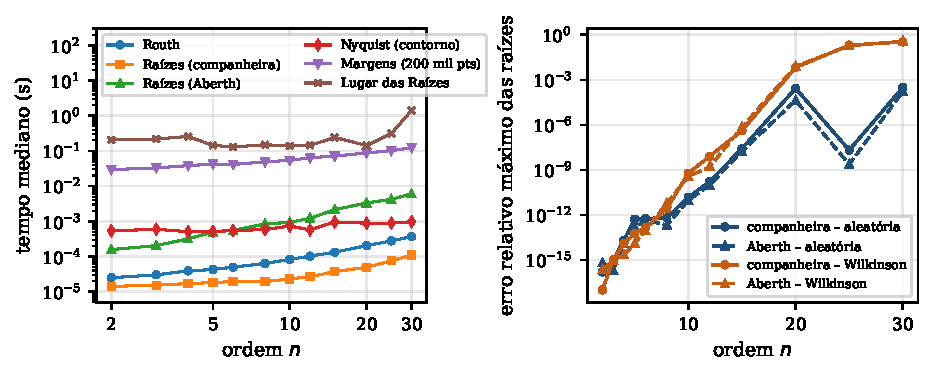
\includegraphics[width=\textwidth]{escalabilidade.pdf}
\caption{Esquerda: tempo mediano por método. Direita: erro relativo máximo das raízes calculadas.}
\label{fig:escala}
\end{figure}

O erro numérico mostra a limitação central dos métodos baseados em raízes. Para a família de Wilkinson, o erro relativo máximo das raízes cresce de $\ErroCompWiCinco$ ($n=5$) para $\ErroCompWiDoisZero$ ($n=20$) com a matriz companheira e de forma semelhante com o Aberth. Isso confirma que a perda de precisão é inerente ao condicionamento do problema, isto é, à sensibilidade das raízes aos coeficientes, e não ao algoritmo \cite{wilkinson1984}. Mesmo assim, o veredito de estabilidade do Routh permaneceu correto em todos os casos testados, pois depende apenas de sinais, e não da localização precisa das raízes.

\subsection{Aplicação: previsão do atraso crítico e montagem HIL}
\label{sec:res-hil}

% Resultados da aplicação (trilha EC): previsão do atraso crítico e montagem HIL no Tinkercad

\textbf{Previsão pelo critério de Nyquist.} Sem atraso, o laço PID do Sistema D tem MF de \MFsemAtraso$^\circ$ em $\omega_{cg}=\WcgD$~rad/s. Logo, o critério prevê instabilidade para um atraso total acima de $\tau_{crit}=\TauCrit$~s, valor confirmado por bissecção sobre o veredito $Z$ do próprio Nyquist (\TauCritBis~s).

\textbf{Gêmeo digital.} A Tabela~\ref{tab:hil-ts} compara a previsão contínua com o menor atraso, em amostras, que torna instável o laço discreto simulado pelo gêmeo, avaliado pela taxa de crescimento da envoltória do erro, sem saturação. Com $T_s=5$~ms, o limite discreto (\TauHilFino~s) praticamente coincide com a previsão corrigida pelo atraso equivalente do ZOH ($\tau_{crit}-T_s/2$). Para períodos maiores, a instabilidade surge cerca de uma amostra antes do previsto, o que é coerente com o atraso de fase adicional da discretização do PID (Euler para trás). Com o período adotado nos \textit{sketches} ($T_s=20$~ms), o limite previsto é de \DcritHil\ amostras (\TauHil~s).

\begin{table}[ht]
\centering
\caption{Atraso crítico: previsão de Nyquist (tempo contínuo) e laço discreto do gêmeo digital.}
\label{tab:hil-ts}
\small
\resizebox{\textwidth}{!}{\begin{tabular}{lccccc}
\hline
$T_s$ (ms) & $d_{crit}$ (amostras) & $\tau$ simulado (s) & $\tau$ Nyquist (s) & $\tau$ Nyquist $- T_s/2$ (s) & Desvio (\%) \\
\hline
5 & 224 & 1{,}120 & 1{,}122 & 1{,}119 & -0{,}18 \\
10 & 111 & 1{,}110 & 1{,}122 & 1{,}117 & -1{,}07 \\
20 & 55 & 1{,}100 & 1{,}122 & 1{,}112 & -1{,}96 \\
50 & 22 & 1{,}100 & 1{,}122 & 1{,}097 & -1{,}96 \\
\hline
\end{tabular}
}
\end{table}

\textbf{Simulação no Tinkercad.} A Figura~\ref{fig:tinkercad-circuito} mostra o circuito montado no Tinkercad Circuits, com os dois Arduinos ligados em cruz pela serial (TX$\to$RX), o potenciômetro que ajusta o atraso, a chave de atraso variável e o LED ``L'' da Planta, que acende quando $|r-y|>0{,}5$ após 10~s. Os ensaios foram executados pelo próprio simulador, e a série completa $y[k]$, $\tau[k]$, $u[k]$ de cada ensaio foi capturada do Monitor Serial da Planta. A Figura~\ref{fig:tinkercad-monitor} mostra a tela do simulador durante o ensaio acima do limite.

\begin{figure}[ht]
\centering
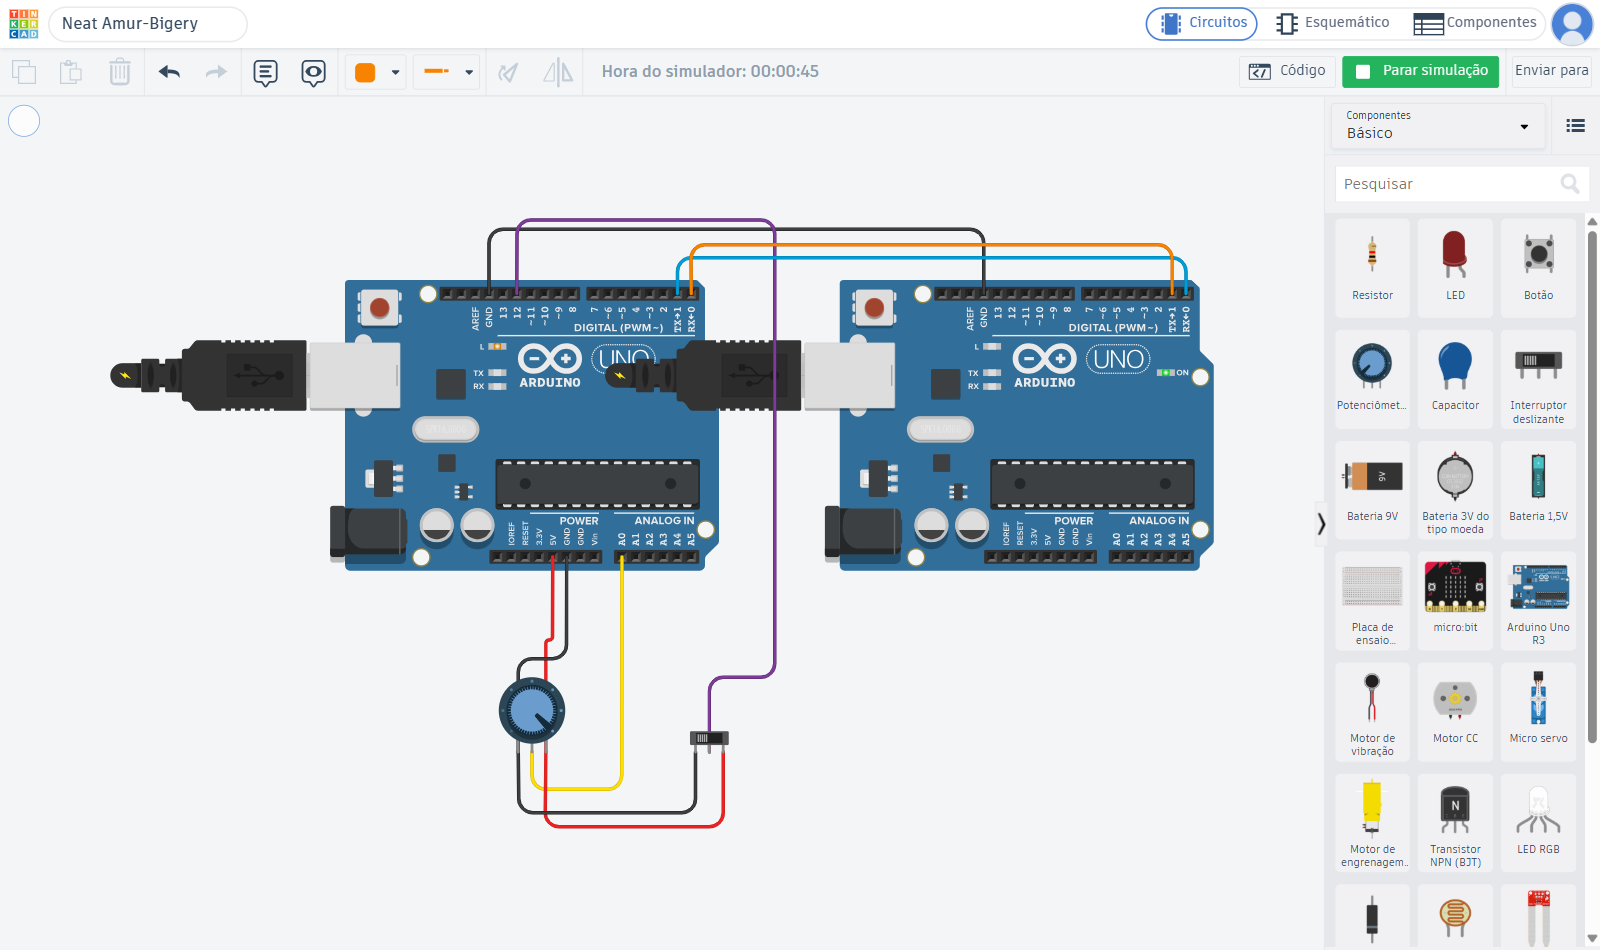
\includegraphics[width=\textwidth,trim=90 110 380 200,clip]{T5_circuito_0.png}
\caption{Circuito HIL simulado no Tinkercad: Arduino ``Planta'' (esquerda) e Arduino ``Controlador'' (direita). Captura feita durante o ensaio T5 ($\tau=1{,}20$~s), com o LED ``L'' da Planta aceso pela oscilação crescente.}
\label{fig:tinkercad-circuito}
\end{figure}

\begin{figure}[ht]
\centering
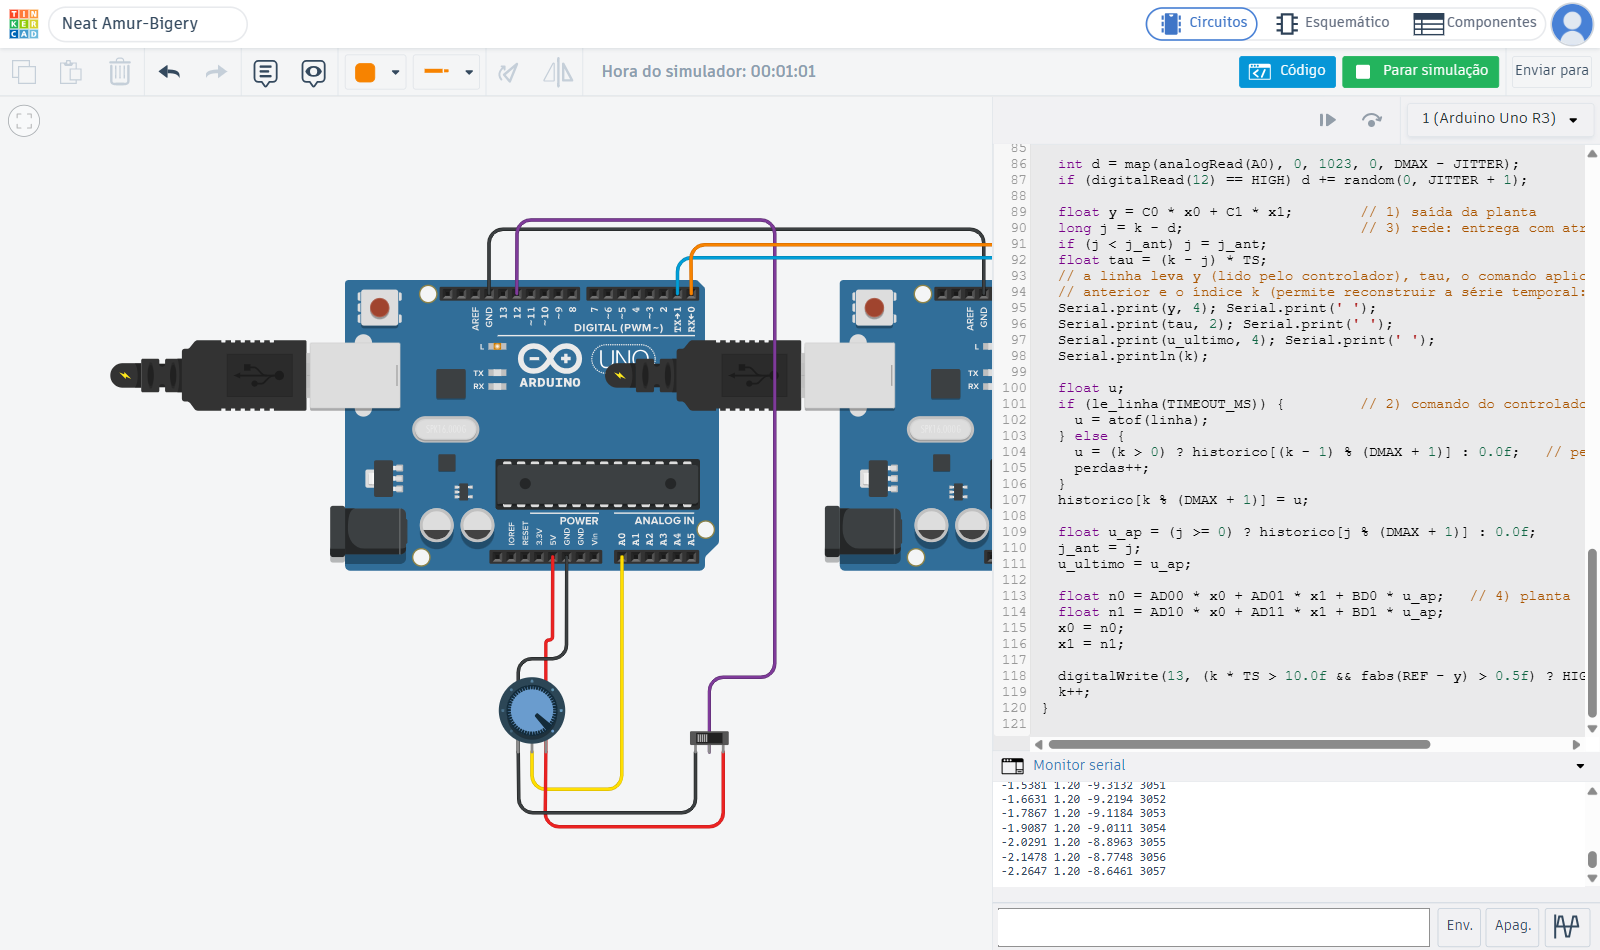
\includegraphics[width=\textwidth]{T5.png}
\caption{Tela do Tinkercad durante o ensaio T5: código da Planta e Monitor Serial com as colunas $y$, $\tau$, $u$ e $k$. O relógio do simulador indica o tempo simulado.}
\label{fig:tinkercad-monitor}
\end{figure}

A Tabela~\ref{tab:tinkercad} e a Figura~\ref{fig:tinkercad-resp} resumem os ensaios. Nos ensaios com atraso fixo, o traço do Tinkercad coincide com o do gêmeo digital, amostra a amostra, com erro máximo de $\ErroTinkMax$, limitado pelas quatro casas decimais da impressão serial. Isso mostra que o comportamento observado no simulador é o do algoritmo especificado, e não um efeito do ambiente. O limite de estabilidade medido no Tinkercad ficou entre $d=\TkQuatroaD$ amostras, que decai com taxa $\TkQuatroaTaxa$~s$^{-1}$, e $d=\TkQuatrobD$ amostras, que cresce com taxa $+\TkQuatrobTaxa$~s$^{-1}$. Esse limite coincide com o do gêmeo e fica a menos de uma amostra (2\%) da previsão do critério de Nyquist em tempo contínuo. O ensaio T5 ($\tau=1{,}20$~s) mostra a oscilação crescente que, com a saturação do atuador, evolui para um ciclo-limite de grande amplitude.

\begin{table}[ht]
\centering
\caption{Ensaios executados no Tinkercad (taxa: crescimento exponencial da envoltória do erro; negativa = estável).}
\label{tab:tinkercad}
\small
\begin{tabular}{lccccc}
\hline
Ensaio & $\tau$ (s) & Pico de $y$ & Taxa (1/s) & Veredito & Erro máx. x gêmeo \\
\hline
T1 & 0{,}00 & 1{,}000 & -- & estável & $9{,}3 \times 10^{-5}$ \\
T2 & 0{,}50 & 1{,}240 & -- & estável & $7{,}4 \times 10^{-5}$ \\
T3 & 1{,}00 & 1{,}822 & -0{,}0467 & estável & $7{,}8 \times 10^{-5}$ \\
T4a & 1{,}08 & 1{,}913 & -0{,}0077 & estável & $8{,}7 \times 10^{-5}$ \\
T4b & 1{,}10 & 2{,}050 & 0{,}0009 & instável & $1{,}2 \times 10^{-4}$ \\
T4c & 1{,}12 & 2{,}687 & 0{,}0091 & instável & $8{,}7 \times 10^{-5}$ \\
T5 & 1{,}20 & 5{,}555 & 0{,}0382 & instável & $1{,}3 \times 10^{-4}$ \\
T6 & 0{,}80--1{,}12 & 1{,}738 & -0{,}1507 & estável & $2{,}3 \times 10^{-4}$ \\
\hline
\end{tabular}

\end{table}

\begin{figure}[ht]
\centering
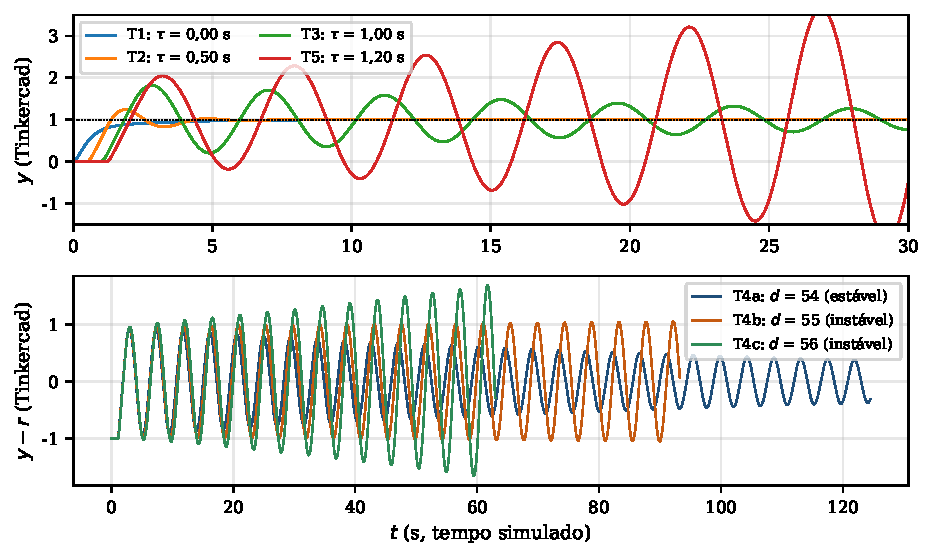
\includegraphics[width=\textwidth]{tinkercad_respostas.pdf}
\caption{Respostas ao degrau medidas no Tinkercad. Acima: ensaios com atraso fixo. Abaixo: erro em torno do limite de estabilidade ($d=54$, $55$ e $56$ amostras).}
\label{fig:tinkercad-resp}
\end{figure}

\textbf{Atraso variável.} No ensaio T6, a chave ativa um atraso sorteado a cada período em $[d,d+20]$ amostras, com base em $d=40$ ($0{,}80$~s). Como os pacotes são entregues em ordem, um pacote não pode ser aplicado antes de um mais antigo. Por isso, o atraso efetivo cresce uma amostra por período até que um sorteio menor libere um pacote mais recente, e permanece próximo do limite inferior da faixa. A estabilidade é, então, governada pelo atraso \emph{mínimo}, e não pelo médio. O gêmeo digital reproduz esse comportamento: com sorteios em $[56,76]$, a malha é instável, enquanto com $[50,70]$ ainda é estável, embora o atraso médio desta última faixa supere o limite para atraso constante. Reproduzindo no gêmeo a mesma sequência de atrasos efetivos registrada no Tinkercad, o erro máximo entre os traços do ensaio T6 foi de $\TkSeisErro$.


% ======================================================================
\section{Discussão}

% Discussão: validação empírica da tabela comparativa do enunciado (Seção 4 do projeto)

O enunciado do projeto propõe uma tabela comparativa entre os quatro métodos e pede que ela seja validada empiricamente. A Tabela~\ref{tab:comparacao} retoma cada característica e indica a evidência obtida neste trabalho.

\begin{table}[ht]
\centering
\caption{Validação empírica da tabela comparativa do enunciado.}
\label{tab:comparacao}
\scriptsize
\begin{tabular}{p{2.3cm}p{2.6cm}p{8.6cm}}
\toprule
Característica & Afirmação do enunciado & Evidência e veredito \\
\midrule
Estabilidade relativa & Nyquist e Bode: sim (MG, MF); Routh: não; Lugar: sim & Confirmada. Nyquist e Bode forneceram MG, MF e margem de atraso. O Routh, sozinho, só classifica; obter a fronteira de ganho exigiu uma varredura em $K$ com bissecção (Tabela~\ref{tab:ganho}). O Lugar fornece os polos e, portanto, amortecimento e frequência natural. \\[1mm]
Sistemas com atraso & Nyquist e Bode tratam de forma exata; Routh e Lugar exigem Padé & Confirmada. A Padé de ordem 1 errou o atraso crítico em \ErroPadeApct\% (para mais, isto é, de forma não conservadora); foram necessárias ordens $\ge 3$ para erro abaixo de $10^{-3}$, ao custo de equações características de grau maior e coeficientes com grande faixa dinâmica (Tabela~\ref{tab:robustez}). \\[1mm]
Instável em malha aberta & Nyquist, Routh e Lugar lidam naturalmente; Bode tem interpretação complexa & Confirmada. No Sistema B, o Nyquist exigiu $N=-1$ e o Routh e o Lugar indicaram um ganho \emph{mínimo}. No Bode, o cruzamento de fase ocorre em $\omega=0$ e a MG é negativa em dB (\MGB~dB), uma leitura que só faz sentido quando se conhece $P$. \\[1mm]
Custo computacional & Routh baixo; Nyquist e Bode moderados; Lugar alto & Confirmada, com ressalvas. O Routh custou de dezenas a centenas de $\mu$s e o Lugar, centenas de ms (o mais caro). O custo do Nyquist (menos de 1~ms) é dominado pelo número de pontos do contorno e quase não depende de $n$. O das margens depende da grade escolhida, e não do método. \\[1mm]
Principal vantagem & Nyquist: atrasos e dados experimentais; Routh: rapidez; Lugar: efeito de $K$; Bode: projeto de compensadores & Coerente com os resultados. O Nyquist foi o único método aplicado sem modificação a todos os sistemas, inclusive com atraso exato, e previu o limite observado na montagem HIL. \\
\bottomrule
\end{tabular}
\end{table}

Três observações complementam a tabela. A primeira é que a concordância de nove casas decimais entre os métodos, nos sistemas racionais, mostra que as diferenças práticas entre eles não estão na resposta, mas no que cada um exige como entrada e no que entrega como saída. A segunda é que o Sistema C evidencia o risco de se apoiar apenas no módulo do Diagrama de Bode: o sistema de fase não mínima e o seu gêmeo de fase mínima são indistinguíveis em $|L(j\omega)|$, mas apenas o primeiro tem ganho limitado (Seção~\ref{sec:res-sistemas}). A terceira é que a robustez numérica não é um detalhe de implementação: um critério ingênuo de ``zero numérico'' no Routh produziu até \RobAbsErro\% de vereditos errados com Padé de ordem alta, sem nenhum aviso. Isso reforça a vantagem do Nyquist, que não precisa expandir o atraso em polinômios.

\textbf{Limitações.} A montagem HIL foi simulada no Tinkercad, e não em hardware físico. O atraso foi emulado por \textit{buffer}, com pacotes sempre entregues em ordem, e a perda de pacotes não foi estudada. Foi avaliado um único ajuste de PID e uma única planta de processo. O cálculo das margens usa uma grade fixa, que, em princípio, poderia deixar de detectar cruzamentos muito próximos entre si. A análise de escalabilidade foi feita em uma única máquina, com tempos de Python interpretado; implementações compiladas mudariam os valores absolutos, mas não as tendências de complexidade.


% ======================================================================
\section{Conclusão}

Este trabalho implementou, sem bibliotecas de controle, uma ferramenta de análise de estabilidade baseada no critério de Nyquist e a comparou com Routh-Hurwitz, Lugar das Raízes e Diagrama de Bode. O módulo de Nyquist trata polos sobre o eixo imaginário por indentação, avalia o atraso de transporte de forma exata e conta os envoltórios por dois algoritmos independentes que sempre concordaram. A ferramenta foi validada por 74 testes unitários, pela comparação com python-control e SciPy e por simulação temporal.

Nos quatro sistemas de teste, os métodos concordaram na fronteira de estabilidade até a nona casa decimal, o que indica que as diferenças práticas estão no que cada método exige e entrega, e não na resposta. O critério de Nyquist foi o único aplicado sem modificação a todos os casos. Com a planta instável em malha aberta, exigiu o envoltório anti-horário previsto pela relação $Z=N+P$. Com o atraso de rede, forneceu o atraso crítico exato de \TauCrit~s, enquanto a aproximação de Padé de primeira ordem errou esse valor em \ErroPadeApct\%, de forma não conservadora.

O estudo de desempenho mostrou que o custo do Nyquist é dominado pela amostragem do contorno e quase não depende da ordem, que o Routh é o mais leve e o Lugar das Raízes o mais caro. A precisão dos métodos baseados em raízes se degrada com a ordem por causa do mau condicionamento: o erro chega a $\ErroCompWiDoisZero$ para o polinômio de Wilkinson de grau 20. Um resultado relevante para a implementação é que um critério ingênuo de ``zero numérico'' no Routh produziu até \RobAbsErro\% de vereditos errados com aproximações de Padé de ordem alta, sem nenhum aviso; o escalonamento de frequência e uma tolerância relativa ao cancelamento eliminaram o problema.

Na aplicação de Engenharia da Computação, um laço PID com atraso de comunicação variável foi executado em dois Arduinos Uno no Tinkercad. O comportamento observado coincidiu amostra a amostra com o gêmeo digital, e o limite de estabilidade medido, entre \TkQuatroaD\ e \TkQuatrobD\ amostras, ficou a menos de uma amostra da previsão do critério de Nyquist. Com atraso variável e entrega em ordem, a estabilidade passou a ser governada pelo atraso mínimo, e não pelo médio.

Como trabalhos futuros, propõem-se: repetir a montagem em hardware físico, com atraso de rede real e perda de pacotes; projetar o controlador a partir da margem de atraso exigida; e substituir a grade fixa do cálculo de margens por um método adaptativo com garantia de detecção de todos os cruzamentos.


\bibliographystyle{sbc}
\bibliography{referencias}

\end{document}
